\documentclass{article}

\textwidth=6.5in
\textheight=8.5in
\voffset=-54pt
\oddsidemargin=0in
\evensidemargin=0in
\setlength{\parskip}{8pt}
\setlength{\parindent}{0pt}

\usepackage{amsmath, amssymb}
\usepackage{ifthen}

\usepackage[inline]{enumitem}
\setlist{topsep=0pt, parsep=8pt}

\usepackage[rgb,table]{xcolor}\convertcolorsUfalse
\usepackage{graphicx}

% change hyperref options
\PassOptionsToPackage{hyphens}{url}
\usepackage[bookmarks,colorlinks,linkcolor=black,citecolor=blue,pdfstartview=FitH,urlcolor=blue]{hyperref}
\hypersetup{pdfpagemode=UseNone}
\usepackage{bookmark}

\usepackage{graphicx}
\usepackage{multicol}
\usepackage{framed}
\usepackage{array}

\usepackage{icomma}

\usepackage{soul}

\usepackage{tikz}
\usetikzlibrary{
  matrix,%
  % enables the snake paths
  decorations.pathmorphing,%
  % enables bigger arrows
  decorations.markings,%
  decorations.pathreplacing,%
  decorations.text,%
  calc,%
  patterns,%
  shapes.geometric,%
  arrows,
  decorations.shapes,
  positioning,
  plotmarks,
  intersections
}
\tikzset{>=latex} % sets default arrow type in tikz
\tikzset{font=\normalsize}
\tikzset{mark size=1.5pt, mark options=thin}
\tikzset{pin distance=4pt,
  every pin edge/.style={<-, thin, shorten <= -2pt}}

\interfootnotelinepenalty=10000
\renewcommand{\thefootnote}{(\arabic{footnote})}

\usepackage{multirow, bigdelim}

% change to \usepackage[sols]{handout} to see solutions
\usepackage{handout}
\renewcommand{\workshopnote}{CA Notes.}    

\newcommand\iscurrentenumi[1]{%
  \ifthenelse{\equal{#1}{\theenumi}}{}{#1}}
\setenumerate[1]{ref=\#\arabic*}
\setenumerate[2]{ref=\protect\iscurrentenumi{\theenumi}(\alph*)}
\newcommand\enumiiprefix[2]{%
  \ifthenelse{{\equal{#1}{\theenumi}}\AND{\equal{#2}{(\alph{enumii})}}}{}{}%
  \ifthenelse{{\equal{#1}{\theenumi}}\AND{\NOT{\equal{#2}{(\alph{enumii})}}}}{#2}{}%
  \ifthenelse{\equal{#1}{\theenumi}}{}{#1#2}%
}
\setenumerate[3]{ref=\protect\enumiiprefix{\theenumi}{(\alph{enumii})}\roman*}

\makeatletter

% underline links               
\let\@href=\href
\renewcommand{\href}[2]{\@href{#1}{\ul{#2}}}

\makeatother

\definecolor{purple}{rgb}{0.5,0,1.0}

\usepackage{fancyhdr}
\lhead{\textcolor{white}{This content is protected and may not be shared, uploaded, or distributed.}}
\rhead{}
\rfoot{\vspace*{\fill}\footnotesize\textcopyright{} \emph{Harvard Math Ma}}
\renewcommand{\headrulewidth}{0pt}
\pagestyle{fancy}
\begin{document}

\htitle{Workshop 8}

\begin{workshop}
  Today's metacognitive focus in on checking your work / thinking about whether it's consistent.

  Give each student an index card, and have them answer the two questions on Slides 1 - 3 and then turn in their answers. The goal of having them turn in their answers is just so they commit to an answer. See the Google Slides for additional notes. 
\end{workshop}

\begin{enumerate}
\item 
  \begin{problem}[\stretch{0.5}]
    Your friend is working on the following problem.

    \begin{quote}
      A bacteria population is growing exponentially. At noon, the population has 400 bacteria. At 2 pm, it has 1200 bacteria. Write a formula giving the bacteria population $t$ hours after noon.
    \end{quote}

    Your friend has gotten the answer $400 \cdot 3^{2t}$. Does their answer work? How can you tell without solving the problem yourself?
  \end{problem} 

\item 

  \begin{workshop}
    Here, the limits are inconsistent with the other information. 
  \end{workshop}

  \begin{problem}[\vfill\newpage]
    Another friend is trying to graph a continuous function $f(x)$. They've found that:
    \begin{itemize}
    \item $f(x)$ is increasing on $(-\infty, -2)$, decreasing on $(-2, 5)$, and increasing on $(5, \infty)$
    \item $f(x)$ is concave down on $(-\infty, 1)$ and concave up on $(1, \infty)$
    \item $\displaystyle \lim_{x \to -\infty} f(x) = \infty$ and $\displaystyle \lim_{x \to \infty} f(x) = 7$.
    \end{itemize}
    They ask for your help sketching the graph of $f$. What would you tell them?
  \end{problem}

\item 
  In each part, fill in the blanks with two consecutive integers, and explain your answer.
  \begin{enumerate}

  \item
    \begin{problem}[0.1in]
      $\cfitb{0.5in}{1} < \log_3 7 < \cfitb{0.5in}{2}$
    \end{problem}

  \item \label{estimate-ln2}
    \begin{problem}[0.1in]
      $\cfitb{0.5in}{0} < \ln 2 < \cfitb{0.5in}{1}$
    \end{problem}

  \item
    \begin{problem}[0.1in]
      $\displaystyle \cfitb{0.5in}{-2} < \ln \left( \frac{1}{3} \right) < \cfitb{0.5in}{-1}$
    \end{problem}

  \end{enumerate}

\item  \label{exp-ln-domain-range}
  \begin{enumerate}
  \item \label{exp-ln-basic-facts}
    \begin{problem}
      Which of the following statements are true? Circle all.
      \begin{enumerate}[label=\Alph*.]
      \item You can only raise $e$ to positive powers.
      \item $e$ raised to any power is positive.
      \item You can only take ln of positive numbers.
      \item ln of any number is positive.
      \end{enumerate}
    \end{problem}

  \item
    \begin{problem}[\vfill]
      One thing you could do to check that your answers to \ref{exp-ln-basic-facts} make sense is to think about the graphs of $e^x$ and $\ln x$. On a single set of axes, make a really big sketch of these graphs. (How do they relate to each other?)
    \end{problem}

  \item \label{ln-points}
    \begin{problem}[\nstretch{0.25}]
      Label any intercepts and asymptotes on your graph of $f(x) = \ln x$. In addition, label one point above the $x$-axis and one point below the $x$-axis with exact coordinates.%
    \end{problem}

  \item \label{ln-transformed}
    \begin{problem}[1in]
      On the same axes, sketch the graph of $g(x) = \ln(2x)$ in a different color. How does the graph of $g$ relate to the graph of $f$? (That is, what transformation should you do to the graph of $f$ to get the graph of $g$?) Where do the intercepts, asymptotes, and points you labeled in \ref{ln-points} move to? Label them on the graph. 
    \end{problem}

  \item

    \begin{workshop}
      One good check is to make sure the labeled points on the graph of $g$ actually satisfy the equation $y = \ln(2x)$. For example, if you moved the point $(e, 1)$ to $\left( \dfrac{e}{2}, 1 \right)$, you can check that $\ln \left( 2 \cdot \dfrac{e}{2} \right)$ really is 1. 
    \end{workshop}

    \begin{problem}[\stretch{1.5}]
      How can you check that your answer to \ref{ln-transformed} is reasonable?
    \end{problem}

  \end{enumerate}

\item 

  \begin{workshop}
    We won't have talked about log rules yet, so the goal here is to use exponent rules. For example, in (c), $\dfrac{25}{\sqrt[3]{5}} = \dfrac{5^2}{5^{1/3}} = 5^{2 - 1/3} = 5^{5/3}$, so $\log_5 \left( \dfrac{25}{\sqrt[3]{5}} \right) = \dfrac{5}{3}$.
  \end{workshop}

  Simplify each of the following.

  \begin{enumerate}
  \item
    \begin{problem}[\vfill]
      $\log_2 \left( 2^4 \cdot 2^5 \right)$
    \end{problem}

  \item
    \begin{problem}[\vfill]
      $\log_3 \left( 9 \sqrt{3} \right)$
    \end{problem}

  \item
    \begin{problem}[\vfill]
      $\log_5 \left( \dfrac{25}{\sqrt[3]{5}} \right)$
    \end{problem}

  \item
    \begin{problem}[\vfill\newpage]
      $\log_7 \left( 49^5 \right)$
    \end{problem}

  \end{enumerate}

\item 

  The strength of earthquakes is typically described using the \textbf{Richter scale}. Here's how it works.

  Scientists measure the seismic waves generated by an earthquake, which look like this:
  \begin{center}
    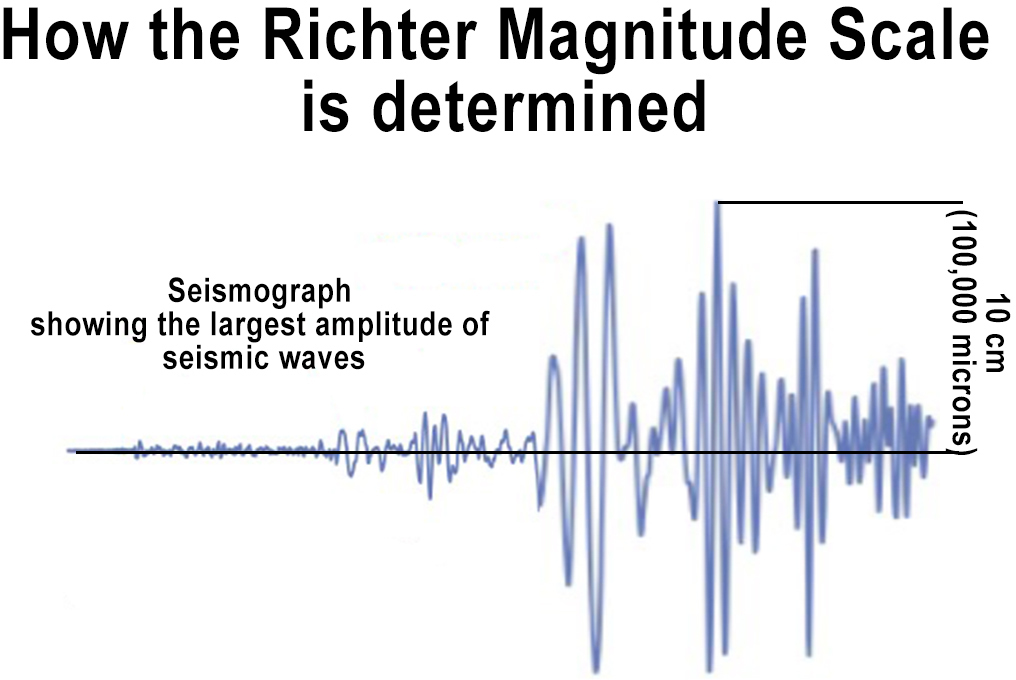
\includegraphics[width=3.5in, trim=0 0 0 1.3in, clip]{images/richter.jpg}

    \emph{Source: \href{https://upload.wikimedia.org/wikipedia/commons/f/f6/How-the-Richter-Magnitude-Scale-is-determined.jpg}{Wikipedia}}
  \end{center}
  They look at the height in microns of the biggest waves (100,000 in the picture above). The Richter scale magnitude is $\log_{10}$ of that height. So, the example above measures \probonly{$\vphantom{\dfrac{1}{1}}$}$\log_{10}(100,000) = \fitb{0.25in}{}$ on the Richter scale.

  \begin{enumerate}
  \item
    \begin{problem}[\vfill]
      Suppose another earthquake measures 6 on the Richter scale. How does the height of its waves compare to the height of the example above? 
    \end{problem}

  \item
    \begin{problem}[\vfill]
      In general, what does a 1 point increase on the Richter scale mean about the height of the seismic waves? 
    \end{problem}

  \item
    \begin{problem}[\vfill\newpage]
      It's possible for an earthquake to be negative on the Richter scale. What does this mean? 
    \end{problem}

  \end{enumerate}

\item 

  \begin{workshop}
    In this problems, students will need to have some idea of how big $\ln 2$ is. They figured this out already in \ref{estimate-ln2}, but it's worthwhile to let them think it through before you point them back there. 
  \end{workshop}

  Let $f(x) = 2x - e^x$.

  \begin{enumerate}
  \item

    \begin{problem}[\vfill]
      Where is $f$ increasing? Where is $f$ decreasing? 
    \end{problem}

  \item
    \begin{problem}[\vfill]
      Where is $f$ concave up? Where is $f$ concave down? 
    \end{problem}

  \item
    \begin{problem}[\vfill]
      Sketch a graph of $f$, labeling any local extrema with their exact coordinates. 
    \end{problem}

  \item

    \begin{problem}[0.25in]
      How many $x$-intercepts does $f$ have? How do you know?
    \end{problem}

    \begin{solution}
      Since the maximum value of $f$ is $2 \ln 2 - 2$ and we saw in \ref{estimate-ln2} that $\ln 2 < 1$, the maximum value of $f$ is negative. Therefore, $f$ has no $x$-intercepts.      
    \end{solution}

  \end{enumerate}

\end{enumerate}
\end{document}
